%% Chong Xing <cxing@ku.edu>
%% Paul Johnson <pauljohn@ku.edu>
%% 20180111
%% The path diagram for semexample/R/Ex-05-SEM/sem-01

% standalone class for individual image to be included in a document
% border=15pt controls the whitespace padding around the diagram
\documentclass[border=15pt]{standalone}
\usepackage{tikz}
\usetikzlibrary{shapes, backgrounds}

\begin{document}

%% ">=latex" sets the arrow head style
%% "semithick" sets the line width (0.6 pt)
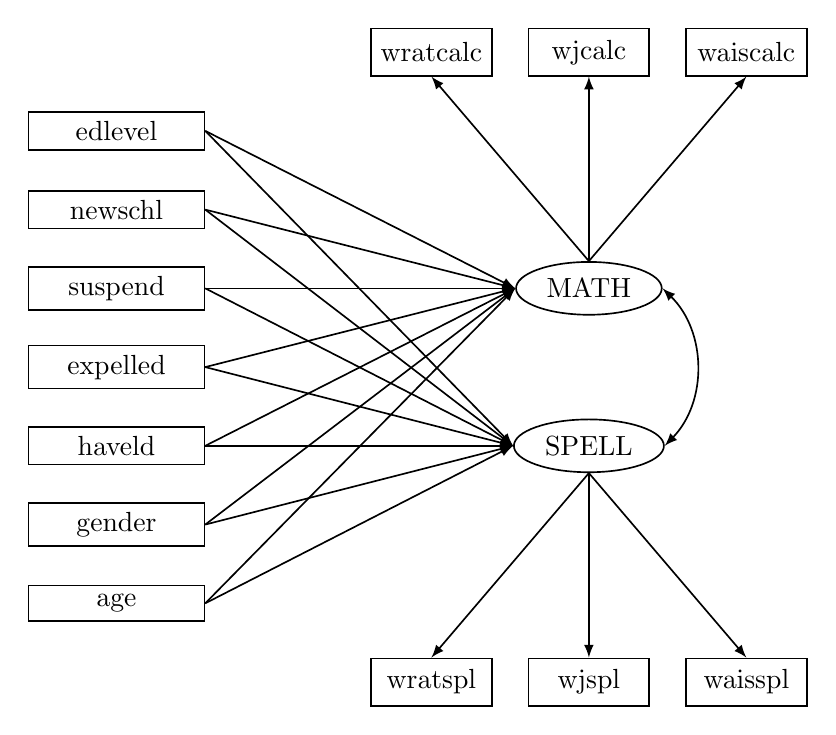
\begin{tikzpicture}[>=latex, semithick];

\node (iv1) at (-6, 3)  [draw, text width=2cm, align=center] {edlevel};
\node (iv2) at (-6, 2)  [draw, text width=2cm, align=center] {newschl};
\node (iv3) at (-6, 1)  [draw, text width=2cm, align=center] {suspend};
\node (iv4) at (-6, 0)  [draw, text width=2cm, align=center] {expelled};
\node (iv5) at (-6, -1) [draw, text width=2cm, align=center] {haveld};
\node (iv6) at (-6, -2) [draw, text width=2cm, align=center] {gender};
\node (iv7) at (-6, -3) [draw, text width=2cm, align=center] {age};

\node (factor1) at (0, 1)  [draw, ellipse, align=center] {MATH};
\node (factor2) at (0, -1) [draw, ellipse, align=center] {SPELL};

\node (indicator1) at (-2, 4)  [draw, text width=1.3cm, align=center, minimum height=0.6cm] {wratcalc};
\node (indicator2) at (0, 4)   [draw, text width=1.3cm, align=center, minimum height=0.6cm] {wjcalc};
\node (indicator3) at (2, 4)   [draw, text width=1.3cm, align=center, minimum height=0.6cm] {waiscalc};
\node (indicator4) at (-2, -4) [draw, text width=1.3cm, align=center, minimum height=0.6cm] {wratspl};
\node (indicator5) at (0, -4)  [draw, text width=1.3cm, align=center, minimum height=0.6cm] {wjspl};
\node (indicator6) at (2, -4)  [draw, text width=1.3cm, align=center, minimum height=0.6cm] {waisspl};

\path[->] (factor1.north) edge (indicator1.south);
\path[->] (factor1.north) edge (indicator2.south);
\path[->] (factor1.north) edge (indicator3.south);

\path[->] (factor2.south) edge (indicator4.north);
\path[->] (factor2.south) edge (indicator5.north);
\path[->] (factor2.south) edge (indicator6.north);

\path[->] (iv1.east) edge (factor1.west);
\path[->] (iv2.east) edge (factor1.west);
\path[->] (iv3.east) edge (factor1.west);
\path[->] (iv4.east) edge (factor1.west);
\path[->] (iv5.east) edge (factor1.west);
\path[->] (iv6.east) edge (factor1.west);
\path[->] (iv7.east) edge (factor1.west);

\path[->] (iv1.east) edge (factor2.west);
\path[->] (iv2.east) edge (factor2.west);
\path[->] (iv3.east) edge (factor2.west);
\path[->] (iv4.east) edge (factor2.west);
\path[->] (iv5.east) edge (factor2.west);
\path[->] (iv6.east) edge (factor2.west);
\path[->] (iv7.east) edge (factor2.west);

\path[<->] (factor1.east) edge [bend left=45] (factor2.east);

\end{tikzpicture}

\end{document}